\subsection{Teil II. Fehlleitung durch den Kritiker}
\label{subsec:Phase2_Misguidance_by_Critic}


\begin{table}[htbp]
\centering
\caption{Stichprobe des Modells Morpheus bei Iteration 2200}
\label{tab:sample_morpheus_2200}
\begin{tabular}{l c}
\hline
\textbf{Parameter} & \textbf{Wert} \\
\hline
Iteration & 2200 \\
Reward & -260.67 \\
Action & [514.42673523, 50.32317324, 4.64697339] \\
Induktivität & \( 5.0 \times 10^{-3} \) \\
Kapazität & \( 10.0 \times 10^{-6} \) \\
\hline
\end{tabular}
\end{table}


Die zweite Phase der Untersuchung offenbarte eine bemerkenswerte Dynamik zwischen dem Akteur und dem Kritiker. Während der Akteur begann, sein Verhalten basierend auf dem Feedback des Kritikers anzupassen, führten diese Änderungen zunächst zu keiner Verbesserung der Zielerreichung. Dies zeigte, dass der Akteur anfänglich den Empfehlungen eines noch nicht ausreichend trainierten Kritikers folgte, was zu suboptimalen Entscheidungen und einer Verschlechterung der Leistung gegenüber dem Referenzwert führte. Der signifikante Abfall des Rewards und die extremen Ausschläge der Ausgangsspannung, die in Abbildung \ref{fig:phase_ii_morpheus} dargestellt sind, verdeutlichen die Konsequenzen der Fehlleitung. Die Ausgangsspannung erreichte Spitzen von bis zu 250 Volt, was in der realen Anwendung wahrscheinlich zu einer Überlastung des Systems geführt hätte. Diese Phase illustriert, wie kritisch es ist, dass der Kritiker präzise und zuverlässige Rückmeldungen liefert, um eine effektive Anpassung des Akteurs zu gewährleisten.Diese Beobachtungen wurden durch die Stichprobe des Modells Morpheus bei Iteration 2200 untermauert, wie in Tabelle \ref{tab:sample_morpheus_2200} dargestellt.


\begin{figure}[htbp]
\centering
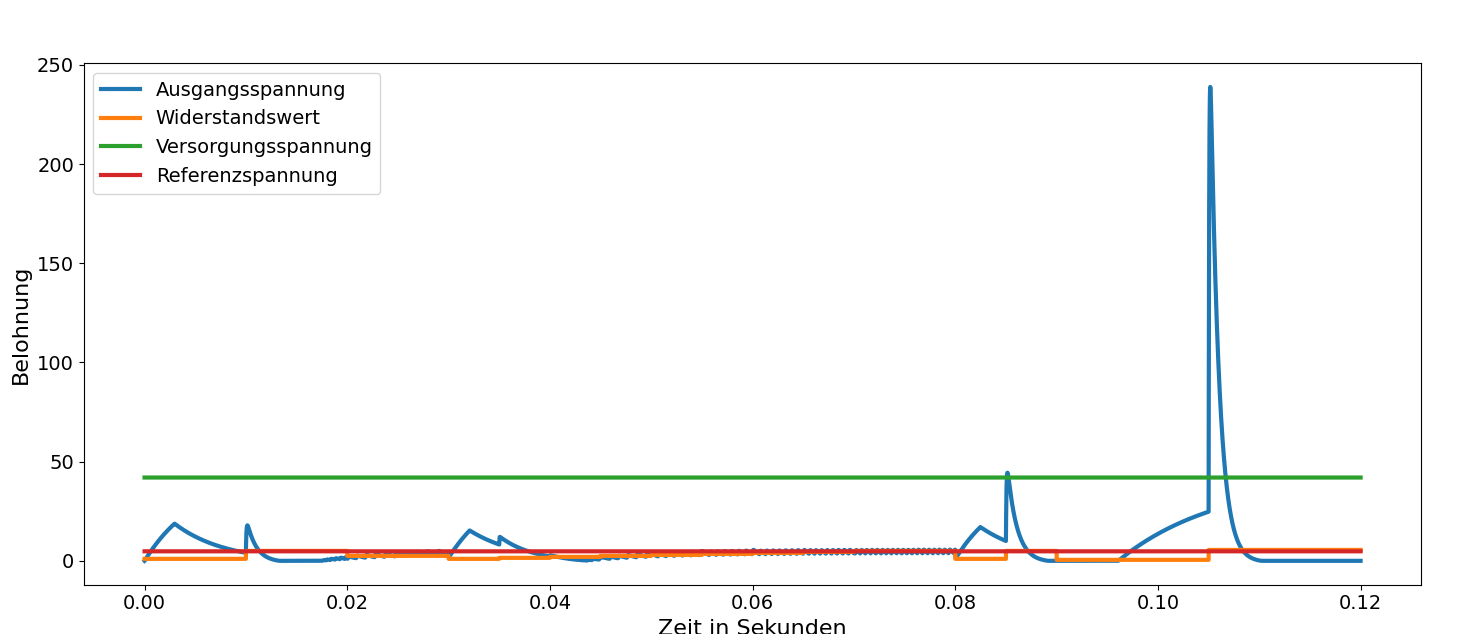
\includegraphics[width=\textwidth]{4Ergebnisse/Phasen/2Phase/TEilII_2.png}
\caption{Auffällige Abweichungen im Regelverhalten des Modells Morpheus während Phase II.}
\label{fig:phase_ii_morpheus}
\end{figure}
